\chapter{Testování a výsledky}
\label{sec:Testing}

Navržená neuronová síť byla testována na sestavě s Linuxovou distribucí Ubuntu 21.10 a obsahující osmijádrový procesor AMD Ryzen 7 5800H, 16 GB RAM a grafickou kartu NVIDIA GeForce RTX 3060 6GB GDDR6.
Právě velikost grafické paměti se při testování sítě ukázala jako největší limitace.
Při akceleraci operací neuronové sítě pomocí grafické karty jsou model i právě zpracovávané data nahrány v grafické paměti, kde za běhu aplikace zabírají kolem pěti GB paměti. 
Na grafické kartě tak zůstávaly řádově stovky MB volné paměti, která bývá navíc z části zabraná systémovými aplikacemi, což nedávalo mnoho místa pro větší zesložitění architektury sítě.

Hlavním cílem testování bylo zjistit, jaký vliv má použití sekvence více snímků na vstupu na přesnost výsledného počtu.
Z toho důvodu bylo natrénováno několik modelů, které se lišily hodnotou parametru \texttt{sequence\_length} udávajícího délku vstupní sekvence, ze které model estimuje počet lidí v jejím posledním obraze.
Stejnou délku měly i sekvence v trénovací množině pomocí kterých byl estimátor natrénován.

Aby se lidskému mozku videosekvence zdály plynulé, jsou při snímání kamerou snímkovány s poměrně vysokou frekvencí. 
Ta může u klasického videa dosahovat například dosahovat hodnoty třicet snímků za sekundu, což znamená, že časový rozdíl mezi jednotlivými snímky je zhruba 0,03 sekundy.
Lidé jsou navíc poměrně pomalu se pohybující stvoření.
Člověk, který jde rychlostí \(4 kmh^{-1}\) se tak za třicetinu sekundy pohne o \(3,5 cm\).
Efekt tohoto pohybu v obraze také bude velmi záviset na tom, jak daleko od kamery se daná osoba nachází. 
V případě, že by scéna byla snímána kamerou s horizontálním rozlišením 1080 pixelů a s objektivem s ekvivalentní ohniskovou vzdáleností \(50 mm\), by člověk jdoucí kolmo ke směru pohledu kamery a vzdálený od ní 10 metrů urazil za třicetinu sekundy vzdálenost ekvivalentní 2,3 pixelů.
Je proto zřejmé, že rozdíly mezi dvěma po sobě jdoucími snímky proto budou minimální a bude v sekvenci tak bude obsaženo velké množství redundantních informací.
Z tohoto důvou byl u trénovaných sítí měněn i parametr \texttt{stride}, který udává krok mezi snímky v sekvenci, a je zkoumán vliv této hodnoty na přesnost výsledku.
Je-li hodnota tohoto parametru rovna jedné, nebudou mezi snímky v sekvenci žádné mezery a budou brány tak, jak se ve vstupním videu nacházejí.
V případě, že má tento parametr hodnotu dva, tak již bude jeden snímek přeskočen a v sekvenci se tak bude nacházet každý druhý snímek ze vstupního videa.

\begin{figure}[h!]
	\centering
	\includegraphics[width=\textwidth]{Figures/testing/Prediction.png}
	\caption{Poslední snímek vstupní sekvence a příslušná hustotní mapa získaná natrénovaným modelem. Nad vstupem se nachází opravdový počet lidí v obraze, zatímco nad hustotní mapou je predikovaný počet získaný sumou hodnot hustotní mapy.}
	\label{fig:Prediction example}
\end{figure}

Výsledné modely byly natrénovány na trénovací části datasetu Fudan-ShanghaiTech a testovány na testovací množině tohoto datasetu.
Tento dataset byl zvolen kvůli velkého celkového množství sekvencí, které mohou být použity pro trénování, relativně vysoké obrazové kvality a rozlišení a zároveň podobnosti s reálnými scénami, na kterých by tento estimátor mohl být nasazený a pomocí kterých by byl testovaný.
Například testování takovéhoto estimátoru natrénovaného s použitím datasetdu DroneCrowd, by bylo v zemích Evropské Unie problematické, jelikož dle evropské legislativy nesmí drony obecně létat nad nezapojenými osobami. \cite{drones_over_people}

Natrénované modely byly trénovány po dobu čtyřiceti epoch, se stejnými hodnotami parametrů.
Jediné, co se u těchto modelů měnilo byla délka vstupní sekvence a velikost kroku mezi jejími snímky.
Při trénování byla pozorováno stejné chování míry chyby sítě, jako je zobrazeno v obrázku \ref{fig:loss_change}, kdy z počátku síť rychle konvergovala k lokálnímu minimu avšak v čím pokročilejší epoše se nacházela, tím nižší byla změna výsledné chyby oproti epoše předchozí.
Čtyřicet epoch proto bylo použito proto, že všechny sítě během nich dokonvergovaly velice blízko lokálního minima.
Při trénování občas také docházelo k tomu, že při počáteční inicializaci vah se síť ocitla v lokálním minimu, ze kterého se již nedokázala vymanit a síť proto nijak více nekonvergovala.
Tato situace se naštěstí dala při trénování odchytnout již po první epoše, kdy výsledná celková chyba sítě byla vyšší, než v případech, kdy síť zdařile konvergovala.

Při průchodu testovací množiny byly zaznamenávány očekávané hodnoty pro každý vstup a výsledné hodnoty získané pomocí testovaného modelu.
Na základě těchto výsledků byly vypočítány hodnoty MAE (Mean Absolute Error), RMSE (Root Mean Squared Error) a MAPE (Mean Absolute Percentage Error), pomocí kterých může být porovnána přesnost modelů.
Hodnota MAE je průměrem absolutních hodnot rozdílů očekávaných (\(y\)) a predikovaných počtů (\(x\)).
RMSE se spočítá jako odmocnina průměru druhých mocnin rozdílů očekávaných a predikovaných počtů a MAPE je průměrem absolutních hodnot odchylek vyjádřených v procentech.

\begin{equation}
MAE = \frac{\sum_{i=1}^{n} | y_{i} - x_{i} |}{n}
\end{equation}

\begin{equation}
RMSE = \sqrt{\frac{\sum_{i=1}^{n} ( y_{i} - x_{i} )^2}{n}}
\end{equation}

\begin{equation}
MAPE = \frac{\sum_{i=1}^{n} \big| \frac{y_i - x_y}{y_i} \big|}{n}
\end{equation}


\begin{table}[h!]
\centering
\begin{tabular}{|l|l||l|l|l|}
\hline
délka sekvence     & stride & MAE    & RMSE   & MAPE   \\ \hline \hline
1                  & 1      & 3,0552 & 4,5311 & 0,1127 \\ \hline
\multirow{3}{*}{2} & 1      & 2,4268 & 3,2834 & 0,0994 \\ \cline{2-5} 
                   & 3      & 2,6422 & 3,6158 & 0,1020 \\ \cline{2-5} 
                   & 5      & 3,3661 & 4,5137 & 0,1339 \\ \hline
\multirow{3}{*}{3} & 1      & 2,2133 & 2,8569 & 0,0913 \\ \cline{2-5} 
                   & 3      & 2,4771 & 3,3323 & 0,0926 \\ \cline{2-5} 
                   & 5      & 3,3158 & 4,4200 & 0,1305 \\ \hline
\multirow{3}{*}{5} & 1      & 2,4405 & 3,6209 & 0,0964 \\ \cline{2-5} 
                   & 3      & 2,3971 & 3,5780 & 0,0930 \\ \cline{2-5} 
                   & 5      & 4,0362 & 5,4004 & 0,1590 \\ \hline
\end{tabular}
\label{tab:errors}
\caption{Hodnoty chyb natrénovaných estimátorů pro testovací množinu datasetu FDST}
\end{table}


\begin{figure}[h!]
	\centering
	\subfloat[]{\includegraphics[height=0.28\textwidth]{Figures/testing/MAE.png}}
	\subfloat[]{\includegraphics[height=0.28\textwidth]{Figures/testing/RMSE.png}}
	\subfloat[]{\includegraphics[height=0.28\textwidth]{Figures/testing/MAPE.png}}
	\caption{Vizualizace hodnoty chyb natrénovaných estimátorů pro testovací množinu datasetu FDST. První obrázek zobrazuje chybu MAE, druhý RMSE a třetí MAPE}
	\label{fig:heatmaps}
\end{figure}

\begin{figure}[h!]
	\centering
	\subfloat[]{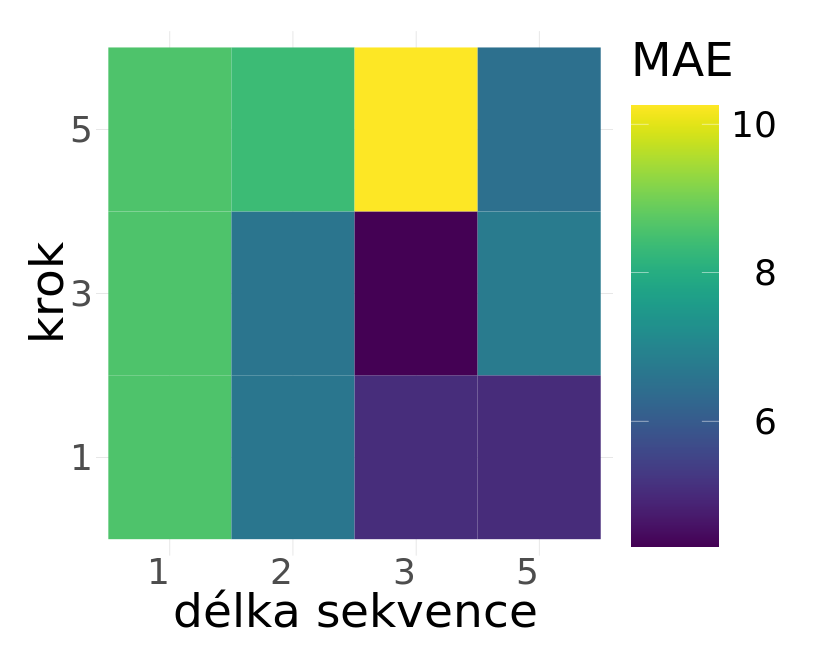
\includegraphics[height=0.28\textwidth]{Figures/testing/MAE_pets.png}}
	\subfloat[]{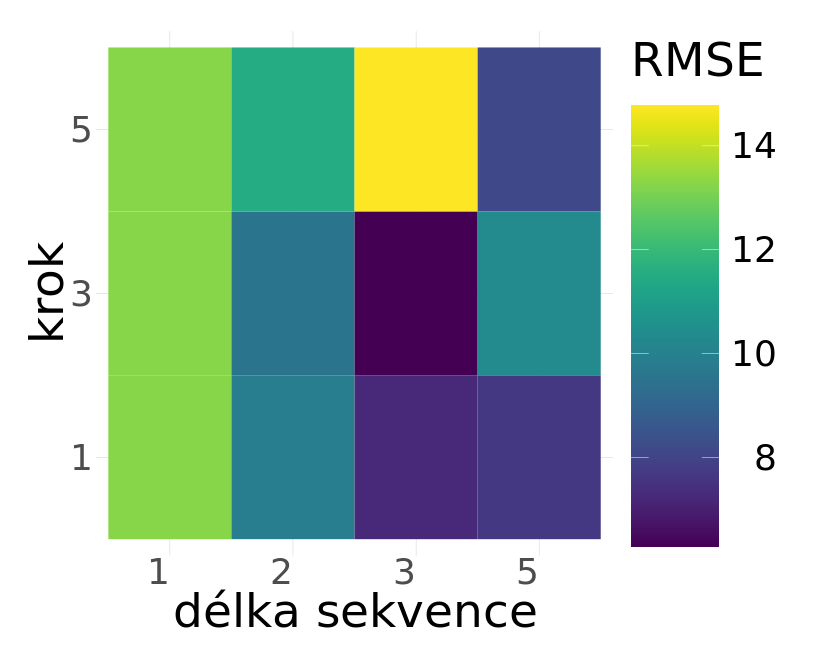
\includegraphics[height=0.28\textwidth]{Figures/testing/RMSE_pets.png}}
	\subfloat[]{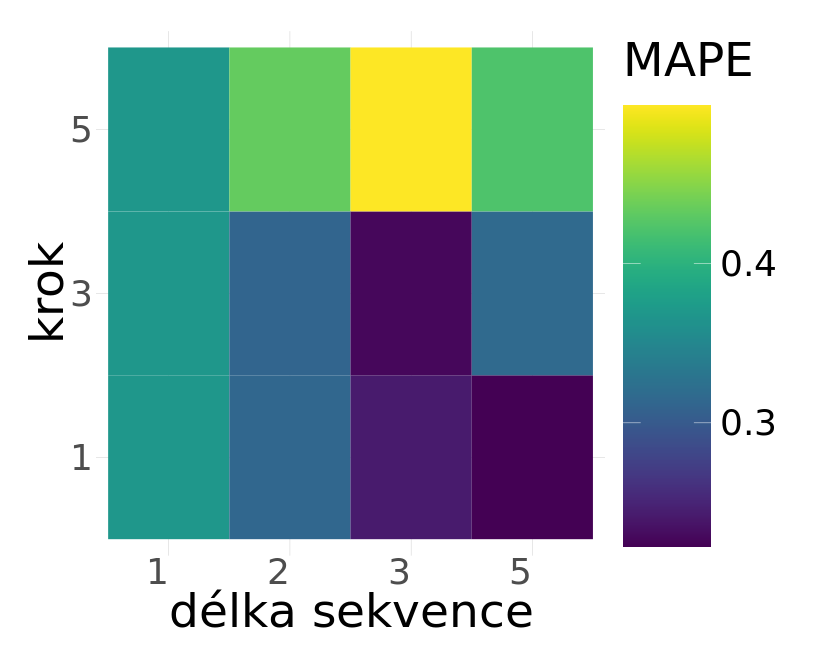
\includegraphics[height=0.28\textwidth]{Figures/testing/MAPE_pets.png}}
	\caption{Vizualizace hodnoty chyb natrénovaných estimátorů při aplikaci na dataset PETS 2009. První obrázek zobrazuje chybu MAE, druhý RMSE a třetí MAPE}
	\label{fig:heatmaps}
\end{figure}




\endinput